\section{Performance}

Our performance tests were done using QEMU/KVM on a 
2-way AMD Quad-core Barcelona system with 8GB of
RAM and a 13 disk fibre channel storage array. Venti
was configured with a 10GB arena and a 512MB isect
and bloom filter. Venti was configured with 32MB of
memory cache, a 32MB bloom cache, and a 64MB isect cache.

For each of our benchmarks, we compared an image
in an Ext3 file system using the QEMU raw block driver
back end, an image exposed through ufs, a user space 9P
file server, using the QEMU block-9P block driver back
end, and then an image stored in Venti exposed through
vdiskfs using the QEMU block-9P block driver back end.

Each benchmark used a fresh Fedora 9 install for
x86\_64. For all benchmarks, we backed the block driver
we were testing with a temporary QCOW2 image. The 
effect of this is that all writes were thrown away. This was
necessary since vdiskfs does not currently support write
operations.

Our first benchmark was a simple operating system
boot measured against wall clock time. The purposes of
this benchmark was to determine if a casual user would
be impacted by the use of a content addressable storage
backed root disk.
Our measurements showed that the when using the QEMU
block-9P driver against a simple 9P block server, there
was no statistically significant difference in boot time
or CPU consumption compared to the QEMU raw block driver.
When using the QEMU block-9P driver against vdiskfs,
we observed a 25% slowdown in boot time along with a 20%
reduction in CPU consumption due to increased latency for
I/O operations.

\begin{figure}[htbp]
\begin{centering}
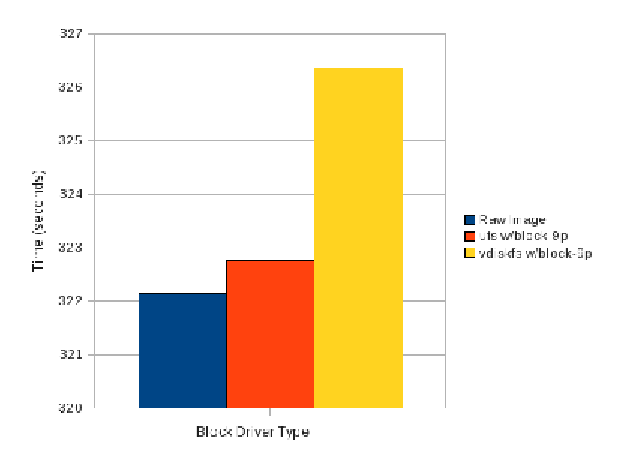
\epsfig{file=bootup.eps, width=2.50in}
\small\itshape
\caption{\small\itshape Boot Time of CAS Storage}
\label{fig:bootup}
\end{centering}
\end{figure}

The second benchmark was a timed \emph{dd} operation.
The transfer size was 1MB and within the guest, direct
I/O was used to eliminate any effects of the guest page
cache. It demonstrates the performance of streaming
read. All benchmarks were done with a warm cache so the
data is being retrieved from the host page cache.

The ufs back end is able to obtain about 111MB/sec using
block-9P.  Since all accesses are being satisfied by the
host page cache, the only limiting factor are additional
copies within ufs and within the socket buffers.

The QEMU raw block driver is able to achieve over
650MB/sec when data is accessed through the host page cache.
We believe it is possible to achieve performance similar to
the QEMU raw block driver through ufs by utilizing splice
in Linux.

\begin{figure}[htbp]
\begin{centering}
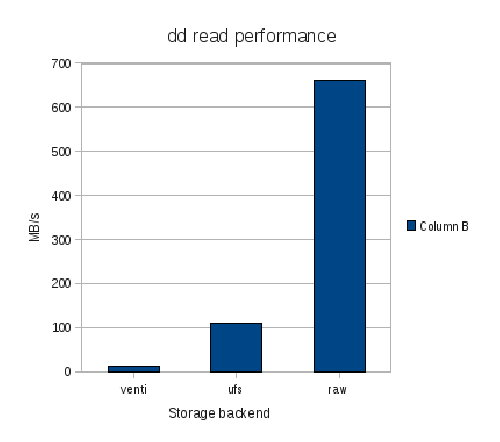
\epsfig{file=dd.eps, width=2.50in}
\small\itshape
\caption{\small\itshape Streaming Read Performance}
\label{fig:streamingread}
\end{centering}
\end{figure}

vdiskfs is only able to obtain about 12MB/sec using
block-9P. 
While this performance may seem disappointing, it
is all we expected from the existing implementation
of Venti and we talk about some approaches to improving
it in Section 5.
